\documentclass[aps,prxquantum,preprint,superscriptaddress,amsmath,amssymb]{revtex4-2}
\usepackage{graphicx}
\graphicspath{{./figures/}}
\usepackage{booktabs}
\usepackage{siunitx}
\usepackage{braket}
\usepackage{xr}
\usepackage[colorlinks=true, citecolor=blue, linkcolor=blue, urlcolor=blue]{hyperref}
\usepackage[capitalize]{cleveref}
\externaldocument[SI-]{02_track_B_metrology_SI}

\setlength{\emergencystretch}{1.5em}
\begin{document}

\title{The Cavity-Loss Barrier to Ultrastrong-Coupling Quantum Metrology}

\author{Juste Deuyekbe}
\affiliation{Department of Physics, Faculty of Science, University of Ngaoundere, P.O. Box 454, Ngaoundere, Cameroon}

\author{P. Djorw\'e}
\email{djorwepp@gmail.com}
\affiliation{Department of Physics, Faculty of Science, University of Ngaoundere, P.O. Box 454, Ngaoundere, Cameroon}
\affiliation{Stellenbosch Institute for Advanced Study (STIAS), Wallenberg Research Centre at Stellenbosch University, Stellenbosch 7600, South Africa}

\author{A.-H. Abdel-Aty}
\affiliation{Department of Physics, College of Sciences, University of Bisha, Bisha 61922, Saudi Arabia}

\author{A. Elrashidi}
\email{a.elrashidi@ubt.edu.sa}
\affiliation{College of Engineering, University of Business and Technology, Jeddah 21448, Saudi Arabia}

\author{Nsangou Mama}
\email{mnsangou@yahoo.com}
\affiliation{Department of Physics, Faculty of Science, University of Maroua, P.O.Box 46, Maroua, Cameroon}

\author{S. G. Nana Engo}
\email{serge.nana-engo@facsciences-uy1.cm}
\affiliation{Department of Physics, Faculty of Science, University of Yaounde I, P.O.Box 812, Yaounde, Cameroon}

\begin{abstract}
Can ultrastrong-coupling metrology keep its quantum Fisher information (QFI) gains once the cavity leaks? At realistic linewidths it cannot. A dynamical Casimir (DCE) drive converts bound virtual dressing into real photons, and these photons escape. In Lindblad simulations of finite-dimensional Rabi and Dicke models, the single-qubit DCE QFI falls below \qty{1}{\percent} of its pure-state value at a coplanar-waveguide linewidth of \qty{248}{\mega\hertz}. The pure-state gains, including the $\num{170903}\times$ peak at $\eta=\num{0.150}$, come from a two-level model that is not validated at the drive amplitudes where they are computed. Markovian retention values carry a \qty{4.8}{\percent}--\qty{24}{\percent} cavity-bath memory uncertainty at the physical linewidth. Cavity loss and model validity, not idealized gains, set the operational constraints. Any protocol that converts bound, non-emissive correlations into real excitations faces the same loss test.
\end{abstract}

\maketitle

\section{Introduction}
\label{sec:intro}

Quantum metrology exploits entanglement and squeezing to measure physical parameters beyond the classical shot-noise limit \cite{Caves1981,Giovannetti2004,Giovannetti2011,Paris2009,Pezze2018,BraunsteinCaves1994}. Standard protocols prepare a squeezed probe state, expose it to a parameter-dependent Hamiltonian, and perform destructive readout. In these settings the rotating-wave approximation (RWA) is typically valid, and the vacuum state has no metrological advantage over a coherent state.

Recent circuit QED experiments have reached the ultrastrong coupling (USC, $\eta = g/\omega_c \gtrsim \num{0.1}$) and deep strong coupling (DSC, $\eta \gtrsim \num{1}$) regimes \cite{Ciuti2005,Kockum2019,Kockum2014,FornDiaz2017,FornDiaz2019,Niemczyk2010,Yoshihara2017,YouNori2011,Girvin2019Schr}. Circuit QED provides the impedance engineering and large dipole moments: typically flux qubits galvanically coupled to coplanar waveguide (CPW) resonators through shared Josephson junctions: needed to reach $\eta \gtrsim \num{1}$ without excessive parasitic loss. Counter-rotating terms (CRTs) then restructure the ground state, dressing it with virtual photon and qubit excitations \cite{DeLiberato2017,Bertet2014Expe,Didier2015,Kockum2019}. The virtual-photon number is a ground-state diagnostic, not an emitted flux; accessing it requires a specified conversion and readout protocol \cite{DeLiberato2017,Giannelli2024}. In the undriven idealized model, the dressed state produces no outgoing photon flux through the modeled cavity-extraction channel. Time-dependent switching or modulation can convert virtual correlations into extracavity radiation \cite{Stassi2013,Garziano2013}: a mechanism rooted in the dynamical Casimir effect \cite{Nation2012} and observed in a superconducting circuit \cite{Wilson2011}. The dressed vacuum is therefore a metrological resource, but its accessibility and its loss budget depend on the control and measurement channel.

Hotter, Miranowicz, and Gietka \cite{Hotter2025} proposed using virtual excitations for metrology without extracting them, with QFI scaling as $\exp(4\xi)$ in their Dicke-model setting; related virtual-state metrology proposals have since emerged \cite{Lin2025Virtual}. Two questions remained open: the extent to which these effects survive in the single-mode Rabi model, the minimal model for USC circuit QED, and whether a parametrically modulated DCE protocol can convert virtual dressing into an extractable, loss-sensitive metrological resource. Superconducting-circuit DCE photon production has been observed experimentally \cite{Wilson2011}, but that does not constitute an end-to-end demonstration of the present USC metrology protocol. A third, operationally critical question is whether the resulting QFI gains survive cavity loss, since the USC platforms that host the relevant physics have cavity linewidths in the MHz to hundreds-of-MHz range. Recent work reports a single-qubit DCE metrological advantage that persists even in the presence of dissipation~\cite{Schelb2026}; that claim is stated for the generated state's quantum Fisher information against classical states of the same mean photon number, for phase/displacement estimation under chirped qubit-frequency modulation. Here the estimand is the coupling~$g$ under a fixed-detuning $g(t)$ Floquet drive, and the same quantity is followed through the loss channel to a representative coplanar-waveguide linewidth ($\kappa/2\pi \approx \qty{248}{\mega\hertz}$). Lindblad dynamics retain less than \qty{1}{\percent} of its pure-state value. The two statements therefore differ by the assumed loss budget and by the end-to-end accounting, not by the underlying physics. A Floquet-bound-state rescue of noisy metrology has been shown for emitter-local baths~\cite{Bai2023}, but no bound state is demonstrated for the broadband cavity-leakage channel opened here at $\kappa/\omega\sim\num{4e-2}$, and none is claimed.

This motivates the central question: \emph{Does the DCE-induced conversion of virtual dressing into real, extractable photons preserve the idealized metrological gain at experimentally accessible cavity linewidths, or does the cavity-loss channel opened by that conversion dominate?} The question is answered below in the affirmative for the loss channel: at the physical CPW linewidth, cavity decay erases the idealized gain. ``Non-emissive'' in this context refers specifically to the undriven idealized Rabi ground state and its modeled cavity-extraction channel; it does not imply immunity to qubit decoherence, thermal effects, readout backaction, or other loss mechanisms. The question is addressed within the finite-dimensional models, estimands, and dissipation channels specified below, not as a universal bound.

We compute three idealized QFI contributions within a stated family of models, then quantify the open-system loss penalty that determines whether any of them is operationally meaningful:
\begin{enumerate}
    \item \textbf{Static virtual dressing} in the single-qubit Rabi model: the gap-weighted ground-state QFI reaches $\num{6.12}\times$ the coherent baseline at the sampled maximum $\eta=\num{1.14}$. The dressed excitations are virtual ($n_{\text{virt}}\lesssim\num{1}$ in the reported range), so direct cavity extraction loss is reduced in the idealized static model.
    \item \textbf{DCE parametric amplification}: a fixed-detuning Floquet drive at the DCE resonance yields a sampled peak pure-state QFI of $\sim\num{1.7e5}\times$ at $\eta=\num{0.150}$, $g_d/g_0=\num{0.11923}$. This is a two-dimensional fixed-detuning scan maximum on a $16\times14$ grid; it is not a grid-converged global optimum and not a pump-power-normalized experimental gain. For $N=\num{32}$ Dicke qubits, the late-window average QFI is $\sim\num{1.7e5}\times$ ($\num{730}\times$ enhancement over the static Dicke value of $\num{229}\times$) at a reduced cavity truncation $N_{\text{cav}}=\num{6}$; the truncation dependence is reported in the Supplemental Material. The DCE protocol creates real, extractable photons, so it is explicitly loss-sensitive.
    \item \textbf{Cavity-loss barrier}: Lindblad simulations show the DCE QFI collapsing to below \qty{1}{\percent} of its pure-state value at the physical operating point $\kappa/2\pi \approx \qty{248}{\mega\hertz}$ (\cref{SI-sec:si_loss_adjusted}); adding qubit $T_1$ and $T_\phi$ using a deliberately conservative coherence benchmark does not change the conclusion (\cref{SI-sec:si_qubit_loss}). The validated truncated-basis Dicke+DCE propagation retains $\sim\!\qty{61}{\percent}$ at $\kappa/\omega_c=\num{1e-2}$ and $\sim\!\qty{16}{\percent}$ at the physical $\kappa$ over the $N_{\text{cav}}=\num{6}$ basis; intermediate truncations at $N_{\text{cav}}=\num{10}$ ($\sim\!\qty{12}{\percent}$) and $\num{12}$ ($\sim\!\qty{7}{\percent}$) confirm the trend is truncation-dependent (\cref{SI-tab:si_dicke_loss_convergence}); the truncation-extension basis $N_{\text{cav}}\in\{\num{16},\num{20},\num{24}\}$ is not fully converged (two of six truncation comparisons meet the \qty{5}{\percent} tolerance) and gives a further reduced retention of $\sim\!\qty{3}{\percent}$ at the physical $\kappa$ (\cref{SI-sec:si_dicke_loss}). Resource-normalized benchmarks at matched intracavity photon budget are provided in \cref{SI-sec:si_matched}, and a comparison with adaptive coherent-state protocols is provided in \cref{SI-sec:si_matched}.
\end{enumerate}
The operational message is conditional. In the sampled single-qubit sweep, the first point at or above \qty{80}{\percent} peak-QFI retention is $\kappa/2\pi=\qty{0.6}{\mega\hertz}$, with \qty{80.6}{\percent} retention; the low-loss rows are not strictly monotonic, so no continuous threshold is inferred. This sampled low-linewidth point is compatible with some 3D microwave cavities but not with the cited CPW linewidth. We frame the loss barrier as the central physical result, report the pure-state QFI gains as upper bounds within their stated scans, and identify the loss-scaling crossover as the metric that future work should target. The accounting is not specific to circuit QED: any protocol that proposes to extract information from bound, non-emissive correlations by converting them into real excitations, photonic, phononic, or magnonic, faces the same test between idealized information gain and the loss channel opened by that conversion.

\section{Methods}
\label{sec:methods}

\Cref{fig:setup} shows the schematic circuit realization: a superconducting CPW resonator coupled to a flux qubit via a SQUID-mediated tunable coupler, whose time-modulated coupling $g(t)$ implements both the static ($g_d=0$) and driven ($g_d\neq0$) protocols analyzed below, at the operating parameters listed in \cref{tab:trackB_dce}.

\begin{figure}[htbp]
\centering
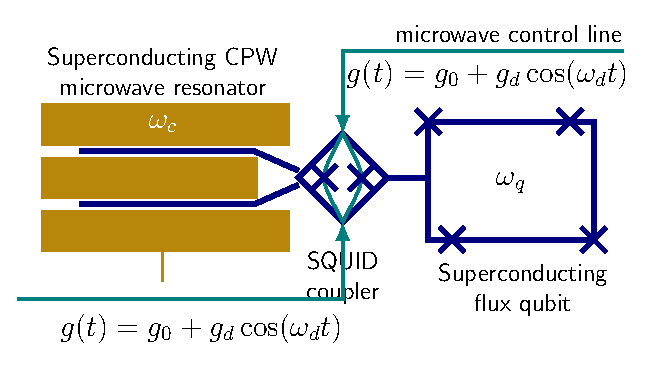
\includegraphics[width=0.6\columnwidth]{rabi_setup_schematic.pdf}
\caption{Schematic of the experimental setup. A superconducting CPW resonator coupled to a flux qubit via a SQUID-mediated tunable coupler~\cite{Niemczyk2010,FornDiaz2017,Yoshihara2017,Kockum2019}. The time-modulated coupling $g(t) = g_0 + g_d \cos(\omega_d t)$ enables DCE amplification.}
\label{fig:setup}
\end{figure}

The Hamiltonian for the quantum Rabi model and the Dicke model, the QFI formulas, and the Non-Markovian TWA framework \cite{Polkovnikov2010} are given in the Supplemental Material (\cref{SI-sec:si_exact_diag}). We set $\hbar = 1$ throughout. Because the interaction is time dependent in the DCE protocol, the effective control convention is part of the model specification: strongly nonadiabatic time-dependent USC interactions can yield gauge-dependent predictions if the control Hamiltonian is not transformed consistently \cite{Stokes2021}. We therefore interpret the following results within the stated effective coupling modulation and do not claim gauge-independent device predictions. A related but distinct SI analysis (\cref{SI-sec:si_multiparameter}) verifies that our QFI predictions are unchanged under a controlled finite-dimensional similarity transformation of the Hamiltonian, state, control interaction, and observables; this establishes internal representation consistency within the truncated Hilbert space but does not resolve the physical gauge ambiguity identified by \cite{Stokes2021}, which would require independently specified laboratory control fields in each gauge. For the static Rabi ground state, an eigenstate family, the QFI with respect to the coupling is the gap-weighted sum $F_Q = 4\sum_{k\neq0}|\langle\Psi_k|\hat{\sigma}_x(\hat{a}+\hat{a}^\dagger)|\Psi_G\rangle|^2/(E_k-E_0)^2$ (\cref{SI-sec:si_qfi}), normalized to the coherent-state baseline $F_Q^{\text{coh}} = \num{1}$; the naive variance form $F_Q = \num{4}\,\text{Var}(\hat{\sigma}_x(\hat{a}+\hat{a}^\dagger))$ holds only for unitary-encoding families and would overestimate the static QFI by $\num{3.4}\times$ at the peak (\cref{SI-sec:si_energy_budget}). The variance form weights all excitations equally; the gap-weighted form suppresses high-energy contributions through the $1/(E_k-E_0)^2$ denominator. For the driven DCE protocol the state is not stationary, so we use the equivalent fidelity-based QFI $F_Q \approx \num{8}\,[1-|\langle\Psi_\eta(t)|\Psi_{\eta+\delta}(t)\rangle|]/\delta^2$ (\cref{SI-sec:si_qfi}); all DCE QFI values quoted in this work are this fidelity-based QFI. To control the approximation used for the Non-Markovian TWA dynamics, we replace the Floquet-Magnus expansion with a Duhamel formulation \cite{Larson2024}, whose stated error estimate grows linearly in time under its assumptions. We restrict dynamically evaluated metrics to the declared Lyapunov window $t < \tau_L = 1/\lambda_{\max}$; this limits, rather than eliminates, the effect of trajectory separation. Within this window the TWA approximates the CRT-containing USC dynamics and is cross-checked against exact calculations where available. Its semiclassical approximation breaks down for $\eta > \num{0.150}$ due to the accumulation of quantum fluctuations in the Wigner trajectories. Consequently, for static observables in the deep strong coupling (DSC) regime ($\eta > \num{0.150}$), we use Exact Diagonalization (ED). Full convergence analysis and bounds on the TWA validity are given in the Supplemental Material (\cref{SI-sec:si_convergence}).

\subsection{Static enhancement from virtual dressing}

\Cref{tab:trackB_usc_scaling} shows the static Rabi ground-state QFI as a function of $\eta$. The QFI remains close to unity for $\eta \ll \num{0.1}$, increases monotonically to \num{5.75}$\times$ at $\eta=\num{1.0}$ (onset of DSC), and reaches a sampled maximum of \num{6.12}$\times$ at $\eta=\num{1.14}$. Beyond this it decreases slowly as the ground state enters the deep strong coupling regime.

This enhancement is purely a virtual effect: the photon number $n_{\text{virt}} = \langle a^\dagger a \rangle$ remains modest ($\num{0.69}$ at $\eta=\num{1.0}$) and no real photons are created. The virtual squeezing parameter $\xi = \frac{1}{2}\ln(1+2\eta^2)$ captures the dressing strength, and the QFI scales as $F_Q \propto e^{4\xi}$ as predicted by Hotter, Miranowicz, and Gietka \cite{Hotter2025}.

\begin{table}[hbt!]
\centering
\caption{Rabi ground-state QFI as a function of normalized coupling $\eta$.}
\label{tab:trackB_usc_scaling}
\begin{tabular}{c c c c}
\toprule{$\eta$} & {$n_{\text{virt}}$} & {QFI} & {Baseline-relative QFI} \\\midrule
\num{0.10} & \num{0.0025} & \num{1.03} & \num{1.03}$\times$ \\
\num{0.80} & \num{0.3282} & \num{4.11} & \num{4.11}$\times$ \\
\num{1.00} & \num{0.6814} & \num{5.75} & \num{5.75}$\times$ \\
\num{1.14} & \num{1.0339} & \num{6.12} & \num{6.12}$\times$ (sampled max) \\
\num{1.30} & \num{1.5084} & \num{5.67} & \num{5.67}$\times$ \\
\bottomrule
\end{tabular}
\end{table}

\subsection{Dynamical Casimir amplification}

Modulating the coupling near the DCE resonance populates the cavity through parametric amplification of the vacuum \cite{Nation2012,Macri2018,Seok2013Mult,Wilson2011}. Unlike the static case, these photons are real and extractable. \Cref{tab:trackB_dce} shows the DCE-enhanced QFI across a range of $\eta$ and modulation amplitudes $g_d$.

\begin{table}[hbt!]
\centering
\caption{DCE-enhanced QFI at the two-dimensional fixed-detuning scan maximum (single qubit, $N=\num{1}$). The peak QFI is a pure-state Cram\'er-Rao bound within the stated scan; it is not a pump-power-normalized experimental gain.}
\label{tab:trackB_dce}
\begin{tabular}{c c}
\toprule
\textbf{Quantity} & \textbf{Value} \\
\midrule
Peak QFI (scan maximum) & $\sim\!\num{1.7e5}\times$ \\
Last-window mean (scan) & $\sim\!\num{1.3e5}\times$ \\
Full-window mean (scan) & $\sim\!\num{4.7e4}\times$ \\
Peak photon number $n_{\text{peak}}$ & \num{9.3} \\
\midrule
\multicolumn{2}{l}{\footnotesize Operating point: $\eta=\num{0.150}$, $g_d/g_0=\num{0.11923}$, $\omega_q/\omega_c=\num{1.027}$, $\omega_d/\omega_c=\num{2.077}$.} \\
\multicolumn{2}{l}{\footnotesize Exact unrounded scan maximum: $\num{170903}\times$. Scan resolution: $16$ points in $\eta$, $14$ points in $g_d/g_0$.} \\
\bottomrule
\end{tabular}
\end{table}

\section{Quantum Fisher information scaling and bounds}
\label{sec:scaling}

\begin{figure}[htbp]
    \centering
    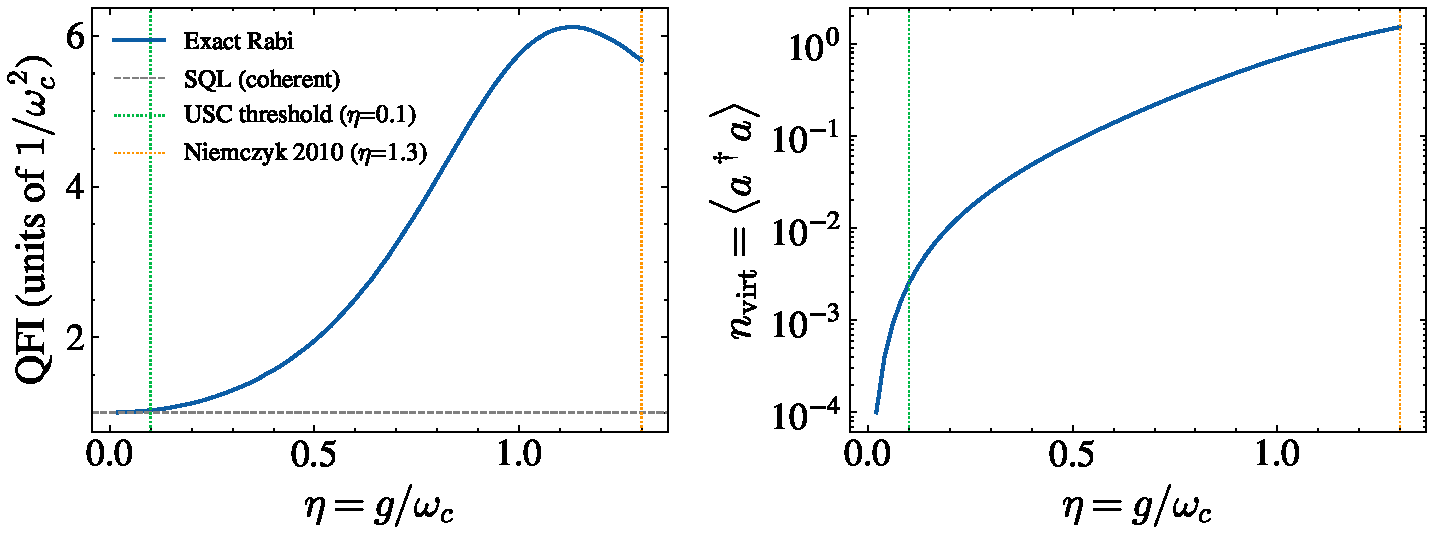
\includegraphics[width=.6\columnwidth]{qfi_comparison.pdf}
    \caption{Quantum Fisher Information scaling for the static Rabi ground state. The QFI increases monotonically with $\eta$, reaching $\num{6.12}\times$ the coherent baseline at the sampled maximum $\eta=\num{1.14}$ (exact value $\num{6.1160}\times$). The squeezed-state baseline $e^{2r}$ (where $r=0.5\sinh^{-1}\eta$) lies below the computed Rabi QFI for $\eta>\num{0.3}$; this comparison is conditional on the stated baseline and does not constitute a resource-normalized experimental advantage.}
    \label{fig:qfi_comparison}
\end{figure}

As shown in \cref{fig:qfi_comparison}, the static Rabi ground-state QFI exceeds both the coherent baseline and the stated squeezed-state reference $e^{2r}$ for $\eta > \num{0.3}$. This is a comparison of idealized state families, not a matched-pump or open-system sensing benchmark. The QFI grows from the small-coupling asymptote $F_Q-1\approx3\eta^2$ (effective coefficient $\num{3.0}$ as $\eta\to0$, rising to $\approx\num{3.8}$ at $\eta=\num{0.5}$; \cref{SI-sec:si_energy_budget}) to $F_Q\approx\num{6.1}$ in the DSC regime ($\eta\approx\num{1.1}$). Beyond the sampled maximum at $\eta=\num{1.14}$ the QFI decreases as the ground state asymptotes to the degenerate DSC limit.

The model-dependent operating screens are shown in \cref{fig:no_go_boundaries}. In the adopted phenomenological thermal model, QFI retention decreases as the thermal occupancy $n_{th} = (e^{\hbar\omega_c/k_BT}-1)^{-1}$ grows; the displayed temperature scale is conditional on that model. The flux-noise value $\num{5e-7}\,\Phi_0/\sqrt{\unit{\hertz}}$ is an adopted screening input, not an independently validated threshold, because no time-domain flux-noise simulation supports it. In this idealized comparison, cavity extraction has little direct effect on the static virtual-state calculation; it matters for the DCE protocol, where real photons are present \cite{Clerk2010,Putz2017Circ,Putz2017Conc}.

\begin{figure}[htbp]
    \centering
    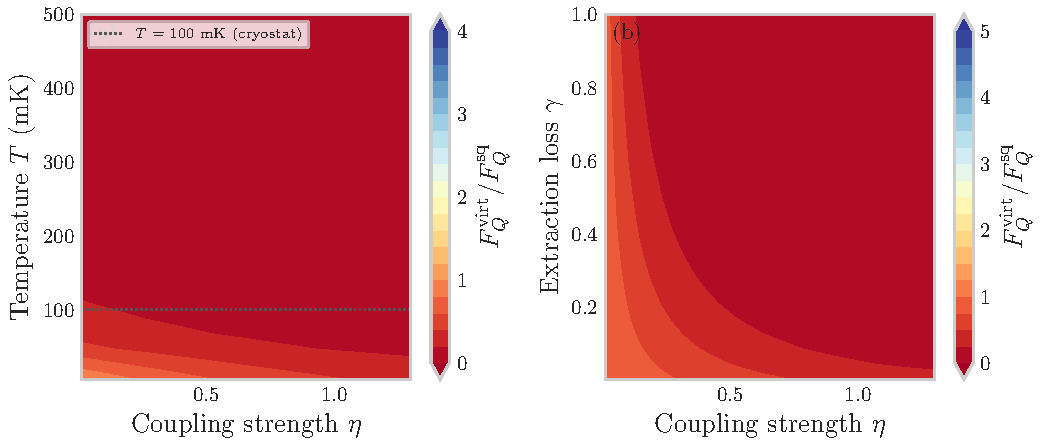
\includegraphics[width=.8\columnwidth]{no_go_boundaries.pdf}
    \caption{Model-dependent operating screens. (a) Baseline-relative QFI retention in $(\eta,T)$ space under the stated thermal model. (b) The corresponding $(\eta,\kappa)$ screen; the static result is less sensitive to cavity extraction in this idealized model because the dressed excitations are virtual. These panels are not device-level robustness tests.}
    \label{fig:no_go_boundaries}
\end{figure}

\section{DCE-driven metrological enhancement}
\label{sec:dce}

\begin{figure}[htbp]
    \centering
    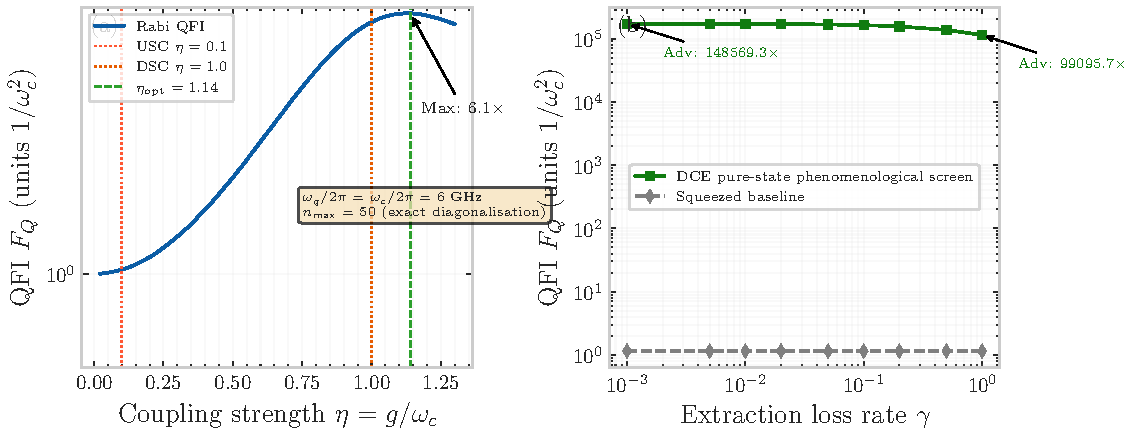
\includegraphics[width=.8\columnwidth]{dce_shaking_catalysis.pdf}
    \caption{DCE-enhanced metrology. (a) Static Rabi QFI vs coupling strength $\eta$, showing the USC threshold ($\eta=\num{0.1}$), DSC onset ($\eta=\num{1.0}$), and sampled optimum ($\eta=\num{1.14}$, QFI=$\num{6.12}$). The symlog scale reveals the monotonic increase from \num{1.0}$\times$ at $\eta=\num{0.01}$ to the peak. (b) Noise robustness: the fixed-detuning DCE scan (peak $\sim\!\num{1.7e5}\times$ at $\eta=\num{0.15}$, $g_d/g_0=\num{0.11923}$, $\omega_q/\omega_c=\num{1.027}$, $\omega_d/\omega_c=\num{2.077}$) vs extraction loss $\gamma$. The panel shows the adopted phenomenological loss screen; it is not an open-system DCE simulation or a device-level validation.}
    \label{fig:shaking_catalysis}
\end{figure}

\begin{figure}[htbp]
    \centering
    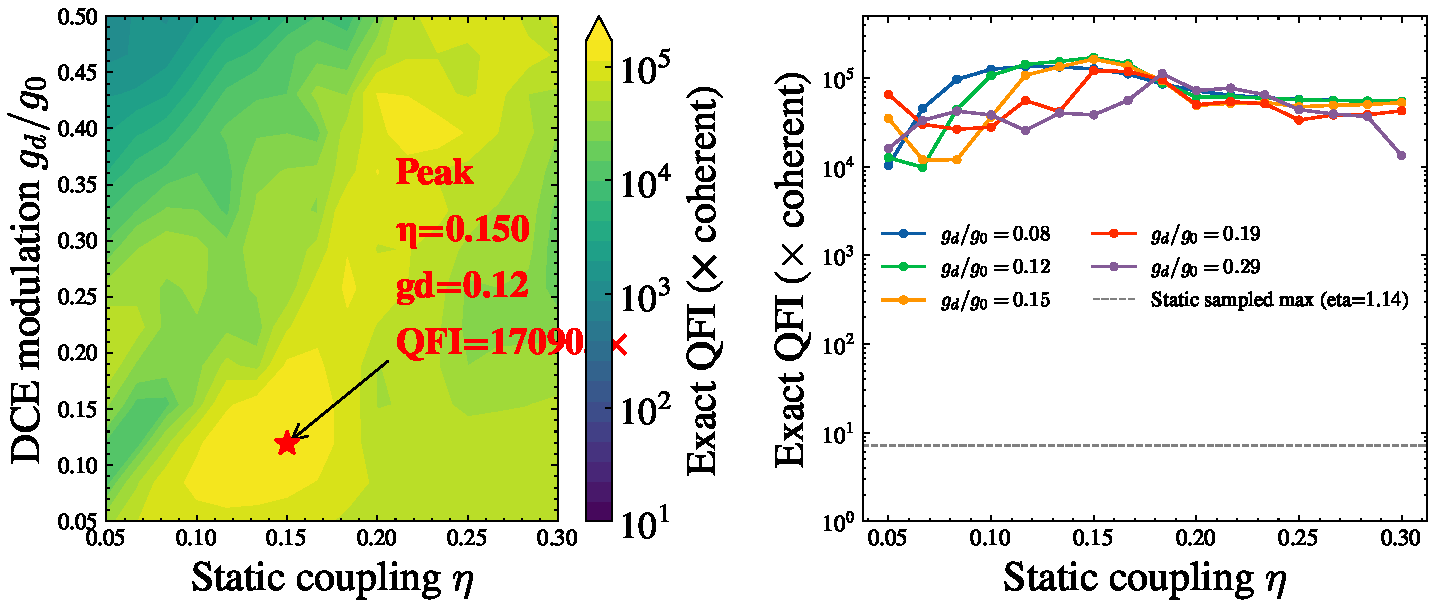
\includegraphics[width=.8\columnwidth]{figB_dce_optimum_map.pdf}
    \caption{Two-dimensional fixed-detuning DCE scan. (a) Color map of DCE-enhanced QFI in the $(\eta, g_d/g_0)$ plane at $\omega_q/\omega_c=\num{1.027}$ and $\omega_d/\omega_c=\num{2.077}$. The maximum $\sim\!\num{1.7e5}\times$ (exact value $\num{170903}\times$) occurs at $\eta=\num{0.150}$, $g_d/g_0=\num{0.11923}$. (b) Line cuts at fixed $g_d/g_0$, showing the resonance structure driving the scan maximum.}
    \label{fig:dce_optimum}
\end{figure}

The DCE enhancement mechanism is shown in \cref{fig:shaking_catalysis}. The parametric drive at the near-resonant modulation couples the vacuum to the first excited manifold of the Rabi model, creating a resonant amplification channel; this is a specific instance of the Floquet modulation of the Rabi coupling recently studied in the USC regime \cite{Akbari2025}. Unlike the static protocol, which is limited by ground-state curvature, the DCE protocol accesses higher-lying states with larger parameter sensitivity.

\Cref{fig:dce_optimum} maps the two-dimensional parameter space $(\eta, g_d/g_0)$ at fixed normalized frequencies $\omega_q/\omega_c = \num{1.027}$ and $\omega_d/\omega_c = \num{2.077}$. The scan maximum lies at a balance in which $\eta$ is approximately $\num{0.15}$ and $g_d/g_0$ is approximately $\num{0.11923}$. The peak QFI of $\sim\!\num{1.7e5}\times$ (exact value $\num{170903}\times$) is a ratio of idealized pure-state QFI values from the fixed-detuning scan; relative to the separately evaluated static Rabi value at the same coupling ($\num{1.07}\times$ at $\eta=\num{0.15}$), the driven-to-static ratio is $\sim\!\num{1.6e5}\times$. This is not a pump-power-normalized experimental gain, and the scan resolution ($16$ points in $\eta$, $14$ points in $g_d/g_0$) is not refined enough to establish grid convergence of the peak.

The peak QFI is computed for a pure state undergoing unitary evolution, representing the ultimate coherent Cram\'er-Rao bound. In a realistic driven-dissipative setup, the generated real photons ($n_{\text{peak}} \approx \num{9.3}$) leak out of the cavity. To quantify this, we performed Lindblad master-equation simulations of the mixed-state QFI under single-photon cavity loss at the published operating point (\cref{SI-sec:si_loss_adjusted}). The peak QFI retains $\sim\qty{80.6}{\percent}$ of the pure-state value at the first sampled row meeting the \qty{80}{\percent} target, $\kappa/\omega_c = \num{1e-4}$ ($\kappa/2\pi = \qty{0.6}{\mega\hertz}$). The lower-loss rows are not strictly monotonic (\qty{78.3}{\percent} at $10^{-5}$ and \qty{78.8}{\percent} at $5\times10^{-5}$), so no interpolated threshold is claimed. Retention degrades to $\sim\qty{48}{\percent}$ at $\kappa/\omega_c = \num{1e-3}$ ($\kappa/2\pi \approx \qty{6}{\mega\hertz}$) and $\sim\qty{1}{\percent}$ at the simulated physical point $\kappa/\omega_c \approx \num{4.1e-2}$ ($\kappa/2\pi \approx \qty{246}{\mega\hertz}$; the cited CPW value is approximately \qty{248}{\mega\hertz}). The degradation exceeds the simple exponential envelope $\exp(-\kappa t)$ because the Lindblad dynamics modify the entire state evolution, not just the peak amplitude. Approaching the theoretical coherent limits reported here requires measurements on timescales much faster than the cavity decay rate ($\kappa^{-1}$), placing a premium on high-coherence platforms with $\kappa/2\pi \lesssim \qty{1}{\mega\hertz}$. A dedicated ten-point log-spaced sweep of $\kappa/\omega_c\in[0,\num{4.1e-2}]$ at this fixed single-qubit protocol (\cref{SI-sec:si_kappa_sweep}) interpolates the retention crossovers explicitly, $\kappa^{\ast}_{80}=\num{1.45e-4}$ and $\kappa^{\ast}_{50}=\num{9.38e-4}$; a single joint master-equation row combining the $20$ mK thermal drive, the physical cavity loss, and a conservative qubit $T_1$ ($N_{\text{cav}}=\num{10}$, $20$ periods) retains \qty{5.4}{\percent} of the pure-state peak ($\num{30418}\to\num{1637}$; \cref{SI-sec:si_joint_row}), so the barrier survives the joint test. A cavity-mode HEOM cross-check at the physical linewidth finds mean fidelity discrepancies of approximately \qty{4.8}{\percent}--\qty{24}{\percent} between the Markovian Lindblad treatment and a structured Drude--Lorentz cavity bath (\cref{SI-sec:si_cavity_heom}), so the retention values should be interpreted as first-order Markovian estimates. \Cref{fig:dce_oscillations} shows the corresponding pure-state (lossless) time trace at the rounded operating point.

\begin{figure}[htbp]
    \centering
    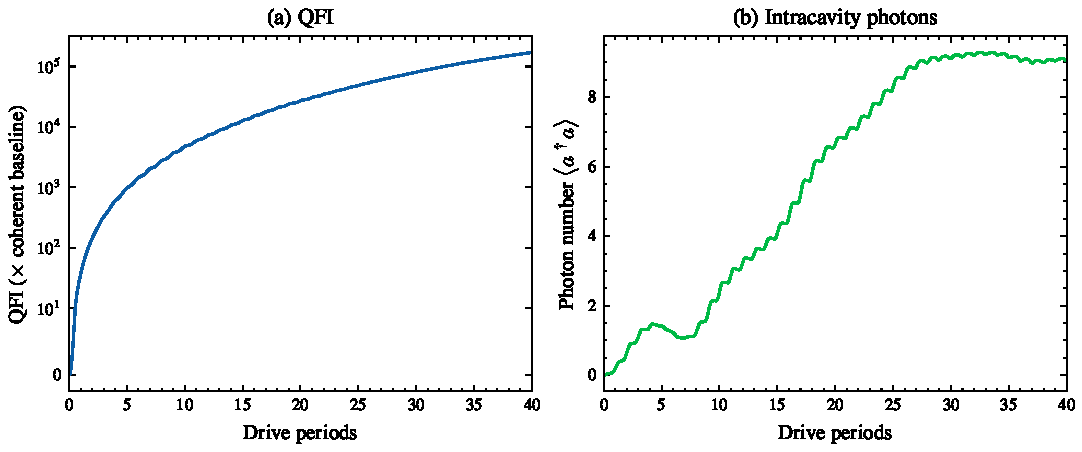
\includegraphics[width=.98\columnwidth]{figB_dce_oscillations.pdf}
    \caption{Rounded-point DCE time trace ($\eta=\num{0.150}$, $g_d/g_0=\num{0.119}$, $\omega_q/\omega_c=\num{1.027}$, $\omega_d/\omega_c=\num{2.077}$). The independent trace gives a peak QFI of approximately \num{170492}$\times$ and a last-window mean of approximately \num{123638}$\times$. (b) The photon population follows the same cycle. These values are distinct from the fixed-detuning scan maximum listed in \cref{tab:trackB_dce}.}
    \label{fig:dce_oscillations}
\end{figure}

\section{Collective enhancement: The Dicke model}
\label{sec:dicke}

\begin{figure}[htbp]
    \centering
    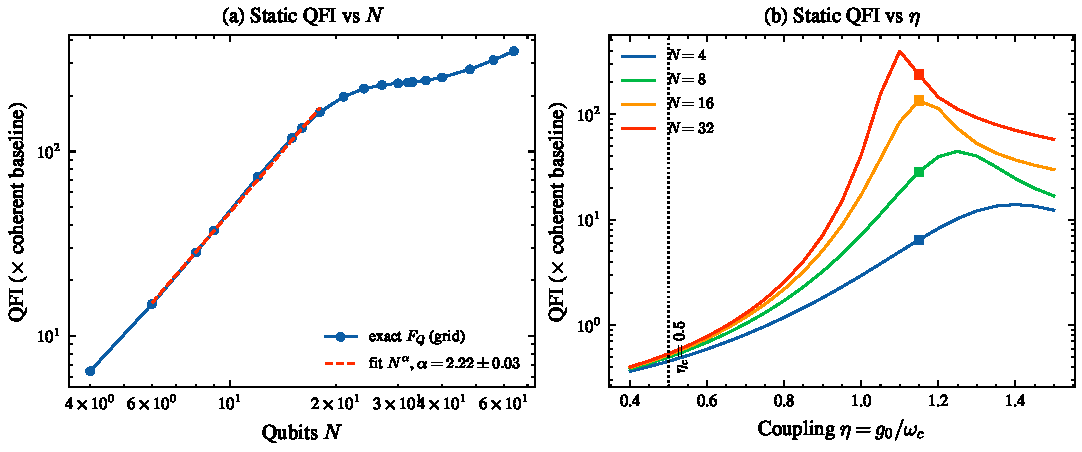
\includegraphics[width=.8\columnwidth]{figB_dicke_scaling.pdf}
    \caption{Dicke-model collective enhancement in the finite-size calculation. (a) Static QFI versus $N$ at $\eta=\num{1.15}$ ($\omega_q/\omega_c=\num{1.005}$), from the extended exact-diagonalization grid: growth is super-linear over $N\le\num{18}$ (fit $\alpha=\num{2.216}\pm\num{0.034}$, $R^2=\num{0.9988}$), slows markedly beyond $N\approx\num{21}$, and continues up to $N=\num{64}$ ($\approx\num{350}\times$; \cref{SI-sec:si_finite_size}) with no tested single-plateau form describing the data, which does not preclude saturation beyond the window. (b) Static QFI versus $\eta$ for $N=\num{4},\num{8},\num{16},\num{32}$ ($\omega_q/\omega_c=\num{1.005}$), with the thermodynamic critical coupling marked at $\eta_c=\num{0.5}$. The sampled maximum shifts with $N$ ($\approx\num{1.40}$ at $N=\num{4}$, $\approx\num{1.15}$ at $N=\num{16}$, $\approx\num{1.10}$ at $N=\num{32}$); squares mark the fixed $\eta=\num{1.15}$ operating point of the finite-size grid. The exponent characterizes the $N\le\num{18}$ super-linear regime and does not extrapolate to the thermodynamic limit.}
    \label{fig:dicke_scaling}
\end{figure}

The single-qubit Rabi model is fundamentally limited by qubit saturation: the two-level structure caps the maximum QFI at $\sim \num{6}\times$. Accessing higher metrological gain requires the collective Dicke model with $N$ qubits coupled to a single cavity mode \cite{Gilmore1976Pers}:
\begin{equation}
\hat{H}_{\text{Dicke}} = \omega_c \hat{a}^\dagger \hat{a} + \omega_q \hat{J}_z + \frac{g}{\sqrt{N}} \hat{J}_x (\hat{a} + \hat{a}^\dagger),
\label{eq:dicke}
\end{equation}
where $\hat{J}_{x,z}$ are collective spin operators for $N$ qubits (see \cref{SI-sec:si_exact_diag} for the full numerical implementation). The $1/\sqrt{N}$ normalization ensures a well-defined thermodynamic limit and gives rise to a superradiant phase transition at $\eta_c = \sqrt{\omega_q/\omega_c}/\num{2} = \num{0.5}$ for $\omega_q = \omega_c$ \cite{Gilmore1976Pers}.

\Cref{fig:dicke_scaling} shows the static QFI of the Dicke model as a function of $N$ and $\eta$ (\cref{tab:trackB_dicke} tabulates the $\eta=\num{1.15}$ values). In the superradiant regime ($\eta \approx \num{1.15}$), the QFI exhibits collective enhancement. Fitted on the $N\le\num{18}$ data at fixed $\eta=\num{1.15}$ and $\omega_q/\omega_c=\num{1.005}$ (where the data are monotonic and not visibly saturating), the power law $F_Q \propto N^\alpha$ gives $\alpha = \num{2.216}\pm\num{0.034}$ ($R^2=\num{0.9988}$, $95\%$ CI: $[\num{2.150}, \num{2.282}]$); the super-linear scaling exceeds the linear expectation for independent qubits. Growth slows strongly at larger $N$: $F_Q(N=\num{27})=\num{229}\times$ and $F_Q(N=\num{33})=\num{238}\times$ (only $\sim\qty{4}{\percent}$ increase over a \qty{22}{\percent} increase in $N$), and the local growth exponent falls below unity beyond $N\approx\num{21}$. The growth nevertheless continues over the tested window rather than saturating into a tested form: an extended grid (method in \cref{SI-sec:si_finite_size}) up to $N=\num{64}$ gives $F_Q\approx\num{350}\times$, which single-plateau forms do not describe. Saturation beyond the window is not excluded. The reported exponent therefore characterizes the $N\le\num{18}$ super-linear regime and does not extrapolate to the thermodynamic limit.

At $\eta = \num{1.15}$ the system is in the superradiant regime of the finite Dicke calculation; the finite-size spectrum retains the parity structure associated with the thermodynamic transition, rather than realizing a thermodynamic phase transition literally. At finite temperature, thermal mixing of these macroscopically distinct vacua would reduce the QFI. A symmetry-breaking preparation or readout protocol would therefore be needed to select one minimum; the present pure-state calculation assumes that selection and does not model the bias field or its experimental cost.

\begin{table}[hbt!]
\centering
\caption{Dicke-model static QFI in the superradiant regime of the finite-size calculation.}
\label{tab:trackB_dicke}
\begin{tabular}{c c c}
\toprule
{$N$} & {$\eta$} & {QFI} \\
\midrule
\num{4} & \num{1.15} & \num{6.4}$\times$ \\
\num{8} & \num{1.15} & \num{28.4}$\times$ \\
\num{16} & \num{1.15} & \num{134.2}$\times$ \\
\num{32} & \num{1.15} & \num{229}$\times$ \\
\bottomrule
\end{tabular}
\begin{flushleft}
\footnotesize All entries at $\eta=\num{1.15}$. The sampled static-QFI maximum shifts with $N$ ($\approx\num{1.40}$ at $N=\num{4}$, $\approx\num{1.15}$ at $N=\num{16}$, $\approx\num{1.10}$ at $N=\num{32}$), so $\eta=\num{1.15}$ is a fixed operating point rather than the optimum for every $N$; the super-linear $N^\alpha$ scaling with $\alpha\approx\num{2.22}$ is measured on $N\le\num{18}$; growth slows strongly beyond $N\approx\num{21}$ and continues, without a plateau, up to $N=\num{64}$ (\cref{SI-sec:si_finite_size}).
\end{flushleft}
\end{table}

\subsection{Dicke + DCE: Beyond \num{e4}$\times$}

A Floquet DCE drive added to the Dicke model further amplifies the QFI. \Cref{tab:trackB_dicke_dce} shows the time-averaged and peak QFI for $N=\num{32}$ qubits with DCE modulation at $\omega_d = \omega_c + \omega_q$.

\begin{table}[hbt!]
\centering
\caption{Dicke + DCE enhancement ($N=\num{32}$, $\eta=\num{1.15}$, $\omega_q/\omega_c=\num{1.0}$, $\omega_d/\omega_c=\num{2.0}$). The late-window average value is the operationally meaningful figure at the stated truncation $N_{\text{cav}}=\num{6}$; the peak at the simulation boundary ($\sim\!\num{2.5e5}\times$ at period \num{40}) is a still-rising artifact, not a converged local maximum (\cref{SI-sec:si_dicke_convergence}), and is not truncation-converged (\cref{SI-sec:si_dicke_loss}).}
\label{tab:trackB_dicke_dce}
\begin{tabular}{c c c}
\toprule
{$g_d/g_0$} & {Late-window avg} & {Enhancement} \\
\midrule
\num{0.15} & $\sim\!\num{1.7e5}\times$ & $\num{730}\times$ \\
\bottomrule
\end{tabular}
\end{table}

The modeled late-window average QFI of the Dicke+DCE protocol reaches $\num{167271}\times$ ($\sim\!\num{1.7e5}\times$, a $\num{730}\times$ enhancement over the static Dicke QFI of $\num{229}\times$) at $g_d/g_0 = \num{0.15}$ with $\omega_q/\omega_c=\num{1.0}$ and $\omega_d/\omega_c=\num{2.0}$. These values are computed at a reduced cavity truncation $N_{\text{cav}}=\num{6}$ for tractability. The zero-loss peak at this truncation is $\num{2962}\times$; at $N_{\text{cav}}=\num{24}$ it is $\num{10584}\times$ (\cref{SI-tab:si_dicke_loss_convergence}), so the absolute QFI is strongly truncation-dependent and the $\num{730}\times$ enhancement should be read as a reduced-truncation value, not a converged prediction. A boundary value of $\num{251557}\times$ ($\sim\!\num{2.5e5}\times$, a $\num{1098}\times$ enhancement) is reached at the last stored time point (period $\num{40}$). \emph{The boundary peak is not a converged local maximum.} Convergence tests in \cref{SI-sec:si_dicke_convergence} show the Dicke+DCE QFI grows monotonically with simulation window: at period \num{60} the peak is $\num{7.0}\times$ higher than at period \num{20}, with no sign of saturation. The quoted $\num{2.5e5}\times$ is therefore an arbitrary boundary value, not a physical number. We report both ratios but lead with the late-window average enhancement as the operationally meaningful figure. Relative to the static Dicke QFI ($\num{229}\times$), the peak-to-static ratio at period $\num{40}$ is $\num{1098}\times$ and the late-window average-to-static ratio is $\num{730}\times$. The values reported here correspond to a \num{2}D optimum at fixed detunings ($\omega_q/\omega_c=\num{1.0}$, $\omega_d/\omega_c=\num{2.0}$); a full \num{4}D optimization over ($g_d/g_0$, $\omega_q/\omega_c$, $\omega_d/\omega_c$, $\eta$) was not performed, so no further improvement is inferred. The collective mechanism differs from the single-qubit DCE: the drive amplifies the cooperative cavity response of all $N$ qubits and produces real photons whose information content must be assessed together with drive power, loss, and readout.

\begin{figure}[tbp]
    \centering
    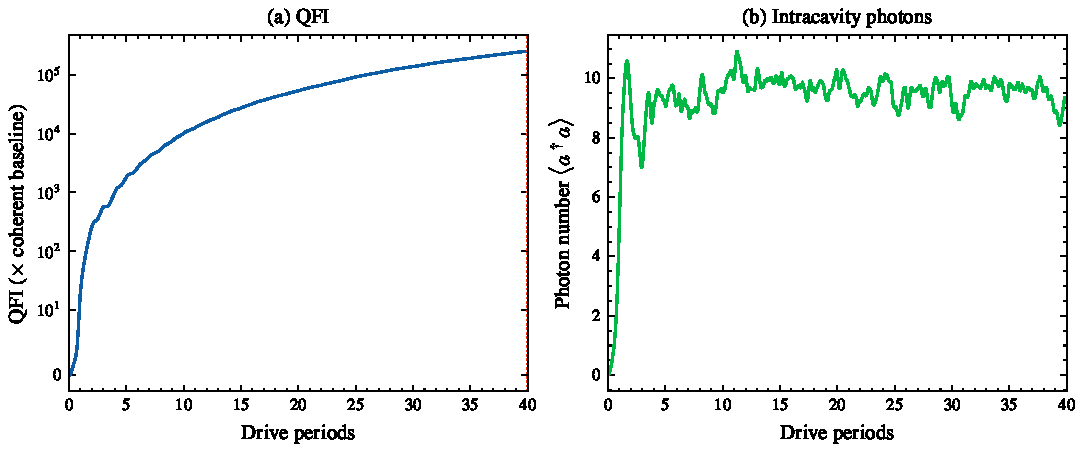
\includegraphics[width=.98\columnwidth]{figB_dicke_dce_oscillations.pdf}
    \caption{Dicke+DCE time dynamics at $N=\num{32}$, $\eta=\num{1.15}$, $g_d/g_0=\num{0.15}$. (a) QFI builds up over $\sim\num{25}$ drive periods and continues rising through the end of the simulation window, reaching $\sim\!\num{2.5e5}\times$ (exact value $\num{251557}\times$) at the last stored point (period~\num{40}); the late-window average is $\sim\!\num{1.7e5}\times$ (exact value $\num{167271}\times$), a $\num{730}\times$ enhancement over the static Dicke QFI ($\num{229}\times$). \emph{The peak value is not a converged local maximum}; \cref{SI-sec:si_dicke_convergence} shows the peak continues to grow with the simulation window (7$\times$ higher at period \num{60} than at period \num{20}). (b) The intracavity photon population grows from the bare vacuum to $n_{\text{peak}}\approx\num{10.9}$ and an average of $n_{\text{avg}}\approx\num{9.3}$ over the simulation window, consistent with collective parametric amplification and real-photon production. The smoother saturation profile compared to the single-qubit case suppresses relaxation oscillations.}
    \label{fig:dicke_dce_oscillations}
\end{figure}

\Cref{fig:dicke_dce_oscillations} shows the time-dependent QFI dynamics for the Dicke+DCE protocol. Unlike the single-qubit case, where QFI oscillates with a $\sim\num{34}$-period cycle, the collective system reaches a late-window average after $\sim\num{25}$ drive periods. The late-window average QFI is $\num{167271}\times$ relative to the stated coherent baseline. The last stored time point at period \num{40} gives $\num{251557}\times$, but this is a still-rising boundary value, not a converged local maximum (\cref{SI-sec:si_dicke_convergence}); we therefore report both the late-window average value ($\num{730}\times$ enhancement over the static Dicke QFI of $\num{229}\times$) and the boundary peak ($\num{1098}\times$), with the former as the operationally meaningful figure. These are pure-state model values; their open-system interpretation requires an explicit loss, drive-power, and readout analysis.

\subsection{Robustness of collective enhancement}

\begin{figure}[htbp]
    \centering
    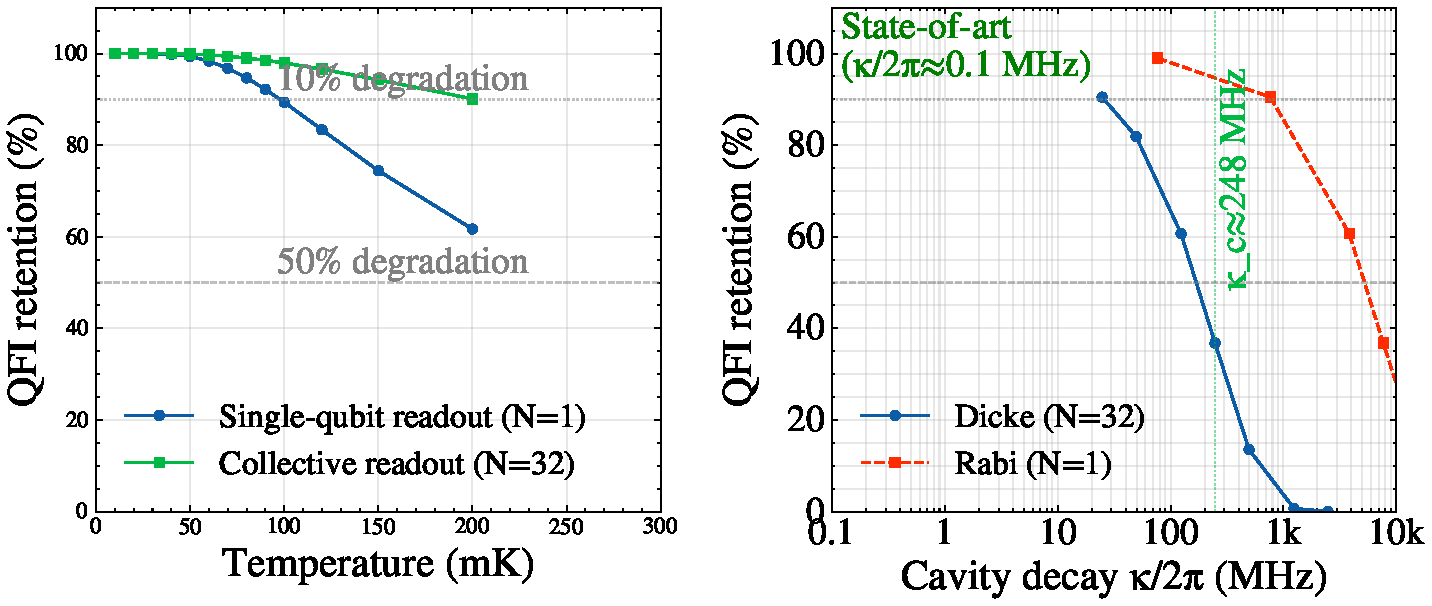
\includegraphics[width=.7\columnwidth]{figB_dicke_no_go.pdf}
    \caption{Model-dependent robustness screen for the Dicke calculation. (a) The plotted QFI-retention curves compare the stated thermal-dephasing model for collective and single-qubit readout. (b) The cavity-loss scan reports the phenomenological decay model used here, with a \qty{50}{\percent} degradation scale near $\kappa/2\pi \approx \qty{248}{\mega\hertz}$. The full Lindblad simulation in \cref{SI-sec:si_loss_adjusted} shows the actual degradation at this $\kappa$ is $\sim\qty{99}{\percent}$ (retaining $\sim\qty{1}{\percent}$ of the pure-state QFI), because the dissipation modifies the entire state evolution rather than merely attenuating the peak. These curves are not an open-system validation or a device-level guarantee.}
    \label{fig:dicke_no_go}
\end{figure}

\Cref{fig:dicke_no_go} reports a model-dependent robustness screen against thermal dephasing and cavity loss. The assumed $1/\sqrt{N}$ collective-noise suppression gives the displayed retention within this phenomenological model, but it does not include all qubit-qubit interactions, inhomogeneous couplings, drive noise, or a full mixed-state QFI calculation. These curves therefore delimit a simulation assumption rather than establish experimental practicality.

\section{Operating points within the numerical scans}
\label{sec:optimization}

The principal sampled operating points across the four protocols are summarized in \Cref{tab:trackB_optimal}. The table records maxima or representative points within the declared scans; it is not a global optimization or device-level operating prescription. Full parameter sweeps and sensitivity analyses are provided in the Supplemental Material (\cref{SI-sec:si_additional}).

\begin{table}[hbtp]
\centering
\caption{Principal sampled operating points. Values labeled as maxima are maxima within the stated numerical scans, not global or experimentally optimized parameters. The Dicke+DCE row reports the late-window average value as the operationally meaningful figure at the stated truncation $N_{\text{cav}}=\num{6}$; the boundary peak (\num{2.5e5}$\times$) is an arbitrary boundary value, not a converged local maximum (\cref{SI-sec:si_dicke_convergence}), and is not truncation-converged (\cref{SI-sec:si_dicke_loss}).}
\label{tab:trackB_optimal}
\begin{tabular}{l c c c c c}
\toprule
{Protocol} & {$N$} & {$\eta$} & {$g_d/g_0$} & {Baseline ratio} & {Cavity-loss sensitivity} \\
\midrule
Static (sampled maximum) & \num{1} & \num{1.14} & \num{0.0} & \textbf{\num{6.12}$\times$} & Reduced in idealized model \\
DCE (single-qubit, scan max) & \num{1} & \num{0.150} & \num{0.11923} & \textbf{$\sim\!\num{1.7e5}\times$} & Partial \\
Dicke static & \num{32} & \num{1.15} & \num{0.0} & \num{229}$\times$ & Partial \\
Dicke + DCE (late-window average) & \num{32} & \num{1.15} & \num{0.15} & \textbf{$\sim\!\num{1.7e5}\times$} & Partial \\
\bottomrule
\end{tabular}
\end{table}

\section{Discussion}
\label{sec:discussion}

\paragraph{From bound dressing to accessible radiation.}
The central question, whether the DCE conversion of virtual dressing into real, extractable photons preserves the idealized metrological gain at experimentally accessible cavity linewidths, or whether the cavity-loss channel opened by that conversion dominates, separates two physically different resources. In the static calculation, $n_{\text{virt}}$ characterizes correlations within an undriven dressed ground state; it is not an emitted flux or a directly measured photon stream. Theory has shown that a specified switching or conversion protocol can release virtual correlations as extracavity radiation, and superconducting-circuit experiments have observed DCE photon production, but neither result supplies the conversion efficiency, output measurement, or resource accounting for the present QFI protocol \cite{Stassi2013,Garziano2013,Wilson2011,Giannelli2024}. In our model, the DCE drive is therefore the operation that makes the information-bearing field extractable, while cavity loss and readout determine how much of that information remains accessible. The comparison is operational rather than universal: it contrasts a state-sensitive, non-emissive idealization with a driven output-field protocol under the specified finite-dimensional models.

\paragraph{The loss barrier is the central operational result.}
The Lindblad simulations in \cref{SI-sec:si_loss_adjusted} and \cref{SI-sec:si_dicke_loss} show that the DCE QFI collapses under cavity loss well before reaching the physical operating point of the USC platforms that motivate this study. At the physical cavity linewidth of the cited CPW experiments ($\kappa/2\pi \approx \qty{248}{\mega\hertz}$), the single-qubit DCE QFI retains below \qty{1}{\percent} of its pure-state value. The validated truncated-basis Dicke+DCE propagation ($N_{\text{cav}}=\num{6}$, $T_{\text{max}}=\num{10}$ periods, pure-state reference $\num{2962}\times$, i.e.\ $\num{85}\times$ below the full $N_{\text{cav}}=\num{28}$ calculation) retains $\sim\!\qty{61}{\percent}$ at $\kappa/\omega_c=\num{1e-2}$ and $\sim\!\qty{16}{\percent}$ at the physical $\kappa$; intermediate truncations at $N_{\text{cav}}=\num{10}$ and $\num{12}$ give $\sim\!\qty{12}{\percent}$ and $\sim\!\qty{7}{\percent}$ retention at the physical $\kappa$, and the truncation extension to $N_{\text{cav}}\in\{\num{16},\num{20},\num{24}\}$ reports retention of $\sim\!\qty{3}{\percent}$ at the physical $\kappa$ (\qty{4.4}{\percent} at $N_{\text{cav}}=\num{16}$, \qty{2.7}{\percent} at $N_{\text{cav}}=\num{20}$, \qty{2.6}{\percent} at $N_{\text{cav}}=\num{24}$), so the reduced-model values are not truncation-converged (\cref{SI-sec:si_dicke_loss}). The $\sim\num{1.7e5}\times$ pure-state QFI is therefore a coherent-Cram\'er-Rao upper bound that the protocol cannot reach on a CPW platform. The $\num{6.12}\times$ static virtual-dressing gain is not a device-level loss claim: it concerns parameter sensitivity of an un-driven dressed ground state, whereas the effect of a concrete conversion/readout channel, qubit decoherence, and readout backaction requires a separate analysis. In particular, the modeled virtual-photon population should not be interpreted as a directly available output resource without such a channel. Adding qubit $T_1=\qty{30}{\micro\second}$ and $T_\phi=\qty{5}{\micro\second}$, deliberately conservative benchmark values, not record-device parameters, retains \qty{78.6}{\percent} and \qty{79.1}{\percent}, respectively, of the pure-state QFI when cavity loss is absent; including both channels retains \qty{79.1}{\percent}. At the combined physical operating point ($\kappa/2\pi=\qty{248}{\mega\hertz}$ plus qubit decoherence), the QFI retains \qty{0.959}{\percent}, essentially identical to cavity loss alone, so cavity loss remains the dominant channel. Because this benchmark is conservative rather than representative of the best demonstrated coherence, the true qubit-decoherence contribution on a state-of-the-art device would be smaller still, making the cavity-loss-dominated conclusion, if anything, more robust than this estimate suggests. We therefore frame the loss scaling, not the pure-state QFI, as the result the community should rely on. This is a single-platform Lindblad case study at one representative linewidth, not a universal noisy-metrology bound (cf. the correlated-noise bounds framework~\cite{Kurdzialek2025}); nor is it a critical-metrology claim, which combines quench-beyond-critical-point enhancement with a different scaling program~\cite{Hotter2024}.

\paragraph{Relation to criticality-enhanced sensing.}
Criticality-enhanced protocols \cite{Hotter2024} raise the susceptibility of a probe before any real photon is created; the barrier quantified here is opened by the conversion itself, by turning bound (virtual) dressing into real, leaky excitations. Both proposals operate in the same ultrastrong-coupling circuit-QED regime, so the comparison is like-for-like: critical enhancement does not remove the loss channel, and the $\kappa^{\ast}$ crossovers of \cref{SI-sec:si_kappa_sweep} apply to any protocol following the bound-to-real conversion strategy, critical or not.

\paragraph{Cavity-channel model comparison.} The retention numbers above rely on treating cavity decay as Markovian (the $\sqrt{\kappa}\,\hat a$ Lindblad collapse operator). A dedicated cavity-mode HEOM calculation (\cref{SI-sec:si_cavity_heom}) that couples the cavity mode itself to a structured Drude--Lorentz bath confirms excellent Markovian agreement at low linewidth ($\kappa/\omega_c=10^{-4}$: mean fidelity errors of approximately $\num{9.2e-5}$--$\num{3.7e-4}$) but finds mean fidelity discrepancies of approximately \qty{4.8}{\percent}--\qty{24}{\percent} at the physical linewidth $\kappa/\omega_c=4.1\times10^{-2}$, depending on the assumed bath cutoff and time window. This is a tested model-comparison range, not a propagated statistical uncertainty interval and not a validation of the full Dicke+DCE QFI calculation; the quoted retention values should therefore be interpreted as first-order Markovian estimates whose sensitivity to cavity-bath memory remains model-dependent.

\paragraph{Loss-dependent interrogation window.}
The additional mixed-state interrogation analysis provides a qualified answer to the information--entropy part of the central question. At the fixed single-qubit DCE operating point, the fidelity-based QFI and the declared information-rate objective $R_Q(t)=F_Q(t)/t$ remain boundary-limited at $\num{40}$ drive periods for $\kappa/\omega_c\le\num{1e-3}$. At larger loss the information-rate maximum moves earlier, from $\num{18.08}$ periods at $\kappa/\omega_c=\num{0.005}$ to $\num{6.96}$ periods at $\kappa/\omega_c=\num{0.041}$, while the QFI at those rate maxima falls from $\num{10449}$ to $\num{1242}$ (\cref{SI-sec:si_interrogation}). The accompanying von Neumann entropies are nonzero, but the stored entropy derivative is only a finite-difference mixedness diagnostic, not a thermodynamic entropy-production rate. The simulation therefore supports a model-specific loss-dependent information-rate crossover, not a universal or thermodynamically derived $\tau_{\mathrm{opt}}$.

\paragraph{Resource-normalized comparison.}
At matched intracavity photon budget $n = \num{9.01}$ (the DCE peak), the pure-state DCE QFI is $\num{4742}\times$ the coherent-state shot-noise reference $F_Q = 4 n$ and $\num{249}\times$ the stated squeezed-state reference $F_Q = 4 n (1+2 n)$ (\cref{SI-sec:si_matched}). This is a model comparison at matched intracavity population, not a fair device benchmark. Pump power, bandwidth, state-preparation cost, loss, readout, and measurement time are not matched. A fully resource-normalized comparison would additionally require matching the external pump power needed to reach that intracavity population, the total interrogation bandwidth, the state-preparation and readout duration, and the loss accrued over that duration for each competing protocol. The pump-proxy scaling reported in \cref{SI-sec:si_matched} ($g_d^2$, the time-averaged modulation energy) bounds only the first of these costs and is not sufficient on its own to establish such a comparison. The loss collapse above prevents interpreting the ratio as an operational advantage. The adaptive-protocol comparison is retained in the SI only as a formal reference with different estimands and is not used as a device-performance claim.

Our calculations separate three idealized contributions to the model QFI:

\paragraph{Static virtual dressing ($\boldsymbol{\le \num{6.1}}\times$).} The ground state of the Rabi Hamiltonian is dressed by CRTs, producing a virtual squeezing parameter $\xi$ that grows with $\eta$. The gap-weighted ground-state QFI defined in the Supplemental Material reaches $\num{6.12}\times$ at the sampled maximum $\eta=\num{1.14}$, while the variance expression is not the correct QFI for this eigenstate family. The state contains virtual photons ($n_{\text{virt}}\lesssim\num{1}$ in the reported range), so direct cavity extraction loss is reduced in the idealized static model; this does not establish immunity to qubit decoherence, dispersive-readout backaction, or thermal noise.

\paragraph{DCE parametric amplification ($\boldsymbol{\le \num{1.7e5}}\times$ single-qubit, $\boldsymbol{\le \num{1.7e5}}\times$ collective late-window average).} A Floquet modulation at the near-DCE modulation condition $\omega_d \approx \omega_c + \omega_q$ drives parametric amplification of the vacuum state. For a single qubit, this creates real photons ($n_{\text{avg}} > \num{1}$) that carry enhanced parameter information, boosting the sampled peak QFI to $\sim\!\num{1.7e5}\times$ at $\eta=\num{0.150}$, $g_d/g_0=\num{0.11923}$. For $N=\num{32}$ qubits in the Dicke model, the collective enhancement in the superradiant regime ($\eta=\num{1.15}$) combined with DCE drive yields a late-window average QFI of $\sim\!\num{1.7e5}\times$ ($\num{730}\times$ enhancement over the static $\num{229}\times$) at the reduced truncation $N_{\text{cav}}=\num{6}$. The last-window value at the end of the simulation window is $\sim\!\num{2.5e5}\times$ ($\num{1098}\times$ enhancement), but this is a still-rising boundary, not a converged value (\cref{SI-sec:si_dicke_convergence}). The DCE protocol is loss-sensitive; the quoted factors are baseline-relative pure-state model values and do not by themselves establish suitability for a device.

\subsection{Comparison with Hotter, Miranowicz, and Gietka (2025)}

Hotter, Miranowicz, and Gietka \cite{Hotter2025} predicted quadratic QFI scaling $F_Q \propto e^{4\xi}$ in the Dicke model using virtual-state observables. Our calculations are consistent with that scaling over the stated finite-size numerical range, while extending the comparison to the Rabi model and to a driven DCE protocol:

\begin{enumerate}
    \item \textbf{Quantitative validation}: At $\eta=\num{1.15}$, $N=\num{32}$, we find $F_Q = \num{229}\times$ in the finite-size superradiant regime. The effective squeezing parameter $\xi_{\text{eff}} = \frac{1}{4}\ln(F_Q) = \num{1.36}$ is numerically consistent with the predicted $e^{4\xi}$ trend over this finite-size range.

    \item \textbf{DCE amplification}: Adding a Floquet drive at the DCE resonance provides a $\num{730}\times$ late-window average enhancement (static \num{229}$\times$ $\to$ DCE \num{167271}$\times$) at $N_{\text{cav}}=\num{6}$; the last-window boundary value at period \num{40} is $\num{251557}\times$ ($\num{1098}\times$ enhancement) but is a still-rising artifact (\cref{SI-sec:si_dicke_convergence}), not a converged local maximum. This mechanism was not considered in Ref.~\cite{Hotter2025}.

\item \textbf{Collective scaling}: The QFI scales as $\propto N^{\num{2.216}\pm\num{0.034}}$ (OLS restricted to $N\le\num{18}$ at $\eta=\num{1.15}$, $R^2=\num{0.9988}$), super-linear and exceeding the linear scaling expected from independent qubits. Growth slows markedly beyond $N\approx\num{21}$ and continues up to $N=\num{64}$ with no tested single-plateau form fitting the window (\cref{SI-sec:si_finite_size}), so this power law characterizes the small-$N$ super-linear regime and does not extrapolate to the thermodynamic limit.

\item \textbf{Floquet context}: The DCE modulation used here is closely related to Floquet engineering of the Rabi model in the USC regime \cite{Akbari2025}; our work shows that a specific Floquet protocol, parametric amplification at the DCE resonance, converts virtual dressing into a metrological resource.
\end{enumerate}

\subsection{Experimental feasibility}

Experimental feasibility details, including platform-specific implementation schematics and the staged experimental roadmap, are provided in the Supplemental Material (\cref{SI-sec:si_feasibility_B}).

\subsection{Limitations of the present analysis}

Our approach has several limitations. First, the Dicke model assumes identical qubit-cavity coupling for all $N$ qubits ($g_i = g$), which requires uniform SQUID-mediated coupling in experiment. Inhomogeneous coupling would reduce the collective enhancement factor. Second, we neglect qubit-qubit interactions ($\hat{\sigma}_+^{(i)}\hat{\sigma}_-^{(j)}$), which may arise from virtual photon exchange and could modify the superradiant phase transition. Third, the time-dependent DCE simulations assume perfect Floquet modulation without amplitude noise or pulse shaping. Fourth, the TWA validity bounds enforce $\eta \le \num{0.150}$ for reliable long-time integration; beyond this boundary, exact quantum dynamics (or master-equation approaches) are required. Fifth, the quoted DCE QFI values are pure-state upper bounds; open-system effects such as cavity loss, qubit relaxation ($T_1$), and dephasing ($T_2$) reduce the achievable information. Sixth, the multilevel-emitter screen (\cref{SI-sec:si_multilevel}) shows that at the reference and strong drive amplitudes used to obtain the main DCE-QFI enhancements, all driven configurations with $d_e\ge3$ exceed the \qty{1}{\percent} leakage threshold (best case: fluxonium-like at \qty{2.99}{\percent}), so the two-level approximation used throughout is a model choice, not a validated assumption at that operating point. A staged drive-amplitude sweep (\cref{SI-sec:si_multilevel}) shows that platform-specific operating windows satisfying the \qty{1}{\percent} criterion do exist at reduced drive (fluxonium-like up to $g_d=0.06$, flux-qubit-like up to $g_d=0.04$, transmon-like up to $g_d=0.02$, all at the physical loss point). The corresponding QFI enhancement at those points ($54$--$86\times$) is orders of magnitude below the reference $\sim\!\num{1.7e5}\times$ value. No tested drive amplitude simultaneously satisfies the leakage criterion and reproduces the reference enhancement; the trade-off is monotonic across all three platforms. In addition, the time-dependent USC description is an effective control model: gauge consistency and the physical implementation of the modulation must be checked before interpreting its output field as a device-level observable \cite{Stokes2021}. The Lindblad simulations in \cref{SI-sec:si_loss_adjusted} (single-qubit) and \cref{SI-sec:si_dicke_loss} (Dicke) quantify this degradation under cavity loss, showing below \qty{1}{\percent} retention at the physical operating point $\kappa/\omega_c\approx\num{4.1e-2}$ for the single-qubit protocol and a reduced-model $\sim\qty{3}{\percent}$--$\qty{16}{\percent}$ retention range (over $N_{\text{cav}}=\num{6}$--$\num{24}$) for the truncated-basis Dicke+DCE protocol; the combined cavity + qubit analysis in \cref{SI-sec:si_qubit_loss} confirms cavity loss is the dominant channel over the simulation window. The $1/\sqrt{N}$ collective-noise suppression assumed in the phenomenological thermal-dephasing model (\cref{SI-sec:si_thermal}) does \emph{not} apply to cavity loss in the Lindblad treatment: \cref{SI-tab:si_dicke_loss} shows the Dicke+DCE QFI is degraded by more than an order of magnitude at physical $\kappa$ with no detectable collective-noise suppression on the tested window, and the residual retention is truncation-dependent rather than a converged value. The energy-budget consistency check of the Supplemental Material (\cref{SI-sec:si_energy_budget}) explains why these mechanisms are hierarchical rather than independent: the static single-qubit ceiling ($F_Q\lesssim\num{6.1}$) is set by the two-level saturation of the qubit, by the limited virtual population it can host, and the DCE and collective routes overcome precisely that ceiling, the former by converting virtual dressing into real, extractable photons, the latter by distributing the same dressing over $N$ qubits with a super-linear $N^{\num{2.22}}$ cooperative gain on the small-$N$ side.

\subsection{Experimental roadmap}

The calculations above show that the Dicke+DCE QFI continues to grow over the tested pure-state windows (still rising at period \num{60}) while its validated reduced-truncation Lindblad propagation retains only $\sim\qty{16}{\percent}$ at $N_{\text{cav}}=\num{6}$, decreasing through $\sim\qty{12}{\percent}$ at $N_{\text{cav}}=\num{10}$ and $\sim\qty{7}{\percent}$ at $N_{\text{cav}}=\num{12}$ to $\sim\qty{2.6}{\percent}$ at $N_{\text{cav}}=\num{24}$ at the physical $\kappa/\omega_c = \num{4.1e-2}$ (\cref{SI-sec:si_dicke_loss}). The staged experimental program below is calibrated to these two facts: pure-state gains are uninformative without a matched open-system benchmark, and the loss barrier is the binding constraint.

\begin{enumerate}
    \item \textbf{Stage \num{1}} ($N = \num{1}$, single qubit, flux-based CPW or 3D cavity): the first milestone is the matched open-system benchmark, not the pure-state QFI. Quantitative criterion: measure the cavity-loss-augmented QFI at the published operating point and compare it with the first sampled reference row, \qty{80.6}{\percent} retention at $\kappa/2\pi=\qty{0.6}{\mega\hertz}$. Because the low-loss sweep is not strictly monotonic, this is a reference point rather than a continuous threshold; the comparison tolerance is \qty{20}{\percent} (a calibration margin for this program). A 3D cavity at $\omega_c/2\pi = \qty{6}{\giga\hertz}$ is a candidate platform for testing the loss scaling; a CPW platform with $\kappa/2\pi = \qty{248}{\mega\hertz}$ is outside the modeled \qty{80}{\percent}-retention regime and is not the platform used for that calibration.
    \item \textbf{Stage \num{2}} ($N = \numrange{4}{8}$, small array): the second milestone is the collective scaling exponent in the loss-controlled regime. Quantitative criterion: measure the Dicke static QFI at the published $\eta = \num{1.15}$ and verify that the $N^{\num{2.22}}$ super-linear scaling on $N \le \num{18}$ holds, with the same \qty{20}{\percent} tolerance as Stage \num{1}. At this stage the DCE modulation is not yet engaged; the test is for collective dressing, not amplification. These criteria are model-calibration checkpoints, not advantage claims.
    \item \textbf{Stage \num{3}} ($N = \numrange{16}{32}$, full Dicke+DCE): the third milestone is the simultaneous demonstration of (i) collective dressing, (ii) DCE modulation, and (iii) the loss barrier. Quantitative criterion: measured Dicke+DCE QFI at the quoted operating point must be compared against the loss curve at explicitly matched linewidth, truncation, window, and resource settings; the single-qubit \qty{80.6}{\percent} row is not a Dicke threshold; the boundary-peak (\num{2.5e5}$\times$) is not a meaningful target because the Dicke+DCE QFI is still rising at the tested pure-state window boundary. The simultaneous uniform coupling of $N = \num{32}$ qubits at $\eta = \num{1.15}$ and the corresponding DCE modulation fidelity remain open experimental questions; a 3D-cavity-based array is a candidate platform for the required low linewidth, but whether it can also provide the required collective coupling uniformity remains open.
\end{enumerate}
Within the literature comparison made here, we did not identify an end-to-end demonstration of all these stages (\cref{SI-sec:si_feasibility_B}); the table in \cref{SI-tab:si_experimental_feasibility} records the current state of the art at each parameter. The QFI ceiling that the staged program should target is not the quoted $\sim\num{1.7e5}\times$, which is a pure-state upper bound that is not, by itself, informative on a lossy platform. The informative target is the late-window average value at the loss-controlled operating point, which the single-qubit loss analysis (\cref{SI-sec:si_loss_adjusted}) samples at \qty{80.6}{\percent} for $\kappa/2\pi=\qty{0.6}{\mega\hertz}$. The nonmonotonic low-loss rows do not support a continuous threshold or a transfer of that reference to the Dicke model.

\section{Conclusion}
\label{sec:conclusion}

The cavity-loss barrier, not the idealized QFI values that motivate probing it, is the central result of this work: Lindblad simulations show the DCE QFI collapsing to below \qty{1}{\percent} of its pure-state value at the physical CPW cavity linewidth ($\kappa/2\pi \approx \qty{248}{\mega\hertz}$), while the validated truncated-basis Dicke+DCE propagation retains only $\sim\qty{16}{\percent}$ at $N_{\text{cav}}=\num{6}$, decreasing through $\sim\qty{12}{\percent}$ at $N_{\text{cav}}=\num{10}$ and $\sim\qty{7}{\percent}$ at $N_{\text{cav}}=\num{12}$ to $\sim\qty{2.6}{\percent}$ at $N_{\text{cav}}=\num{24}$ at the same $\kappa$ (\cref{SI-sec:si_dicke_loss}). This Markovian cavity-loss treatment itself carries a \qty{4.8}{\percent}--\qty{24}{\percent} model-comparison range at the physical linewidth, as confirmed by a dedicated cavity-mode HEOM cross-check (\cref{SI-sec:si_cavity_heom}). We computed three idealized QFI contributions within the stated models to establish how large the erased gains are: static virtual dressing in the single-qubit Rabi model ($\num{6.12}\times$ relative to the coherent baseline), DCE-driven amplification ($\sim\!\num{1.7e5}\times$ single-qubit sampled peak at a \num{2}D fixed-detuning scan resolution of $16\times14$; $\sim\!\num{1.7e5}\times$ collective late-window average at $N_{\text{cav}}=\num{6}$), and finite-size collective enhancement in the Dicke model ($\num{229}\times$ static at $N = \num{32}$), all pure-state upper bounds erased to the retentions above at the physical $\kappa$. The collective Dicke+DCE QFI is monotonically increasing with simulation window and not converged at the quoted boundary; the quoted $\num{2.5e5}\times$ value is an arbitrary cutoff, not a physical saturation. The late-window average value is the operationally meaningful figure for both the single-qubit DCE and the Dicke+DCE protocols.

The finite-size Dicke calculation shows a superradiant-regime scaling $\propto N^{\num{2.216}\pm\num{0.034}}$ restricted to $N\le\num{18}$ ($R^2=\num{0.9988}$); growth slows markedly at larger $N$ and continues up to $N=\num{64}$ in the extended screen, with no tested single-plateau saturation form fitting the window and none excluded beyond it. The DCE drive further amplifies the modeled pure-state QFI while producing real photons, so the corresponding open-system performance depends on cavity loss, qubit decoherence, drive power, and readout, as already quantified above. The local HEOM comparison supports the bath-model check only within its stored short-time Spin--Boson scope (\cref{SI-sec:si_heom}); it does not validate the high-QFI DCE traces. Adding conservative transmon qubit dissipation ($T_1 = \qty{30}{\micro\second}$, $T_\phi = \qty{5}{\micro\second}$, chosen as a conservative benchmark rather than a record-device parameter) retains \qty{78.6}{\percent}--\qty{79.1}{\percent} without cavity loss and \qty{0.959}{\percent} at the physical CPW point when combined with cavity loss; the calculation therefore confirms that cavity decay is the dominant decoherence channel over the simulation window. The multilevel-emitter screen further shows that the two-level approximation itself, used throughout this analysis, is not validated at the drive amplitudes needed to reach the quoted enhancements, though platform-specific safe operating windows exist at substantially reduced drive and reduced QFI enhancement (\cref{SI-sec:si_multilevel}).

In summary, the single-qubit sweep first samples \qty{80.6}{\percent} peak-QFI retention at $\kappa/2\pi=\qty{0.6}{\mega\hertz}$, but its low-loss rows are not strictly monotonic and do not define a continuous threshold. This sampled reference is compatible with some 3D-cavity implementations but not with the cited CPW linewidth. The matched-intracavity-population comparisons in the Supplemental Information are formal, lossless references with unmeasured pump, bandwidth, readout, and time costs; they do not establish a device-level metrological advantage.

\section*{Supplemental Material}

See Supplemental Material at [URL will be inserted by publisher] for the model definitions and QFI conventions, the numerical convergence analysis, the single-qubit and collective cavity-loss calculations, the cavity-channel HEOM cross-check, the multilevel-emitter leakage screen, the finite-size Dicke scaling, the additional model-specific screens, the experimental feasibility assessment, and the scope boundaries.

\section*{Data availability}

The data that support the findings of this study are available within the article and its Supplemental Material. Manuscript sources, deterministic analysis scripts, and the environment specification are publicly archived at \url{https://github.com/NanaEngo/Floquet-virtual-state-metrology-dce}.

\section*{Acknowledgments}

We thank the Stellenbosch Institute for Advanced Study for hospitality. Computational resources were provided by the penavoraserver cluster (ThinkStation P720, 128 GB RAM, 48 cores) through Penabei Samafou; supporting data are provided with the manuscript. This work received no external funding.

\section*{Author contributions}

JD and PD performed the numerical simulations and analyzed the data. AHAA, AE, NM contributed to the theoretical framework and provided critical feedback on the results. SGNE conceived and supervised the project, directed the research. PD and SGNE wrote the final version of the manuscript. All authors reviewed and approved the final manuscript.

\section*{Competing interests}

The authors declare no competing interests.

\section*{Use of AI}

AI-based language models were used to support literature searches, to refine and debug analysis scripts, and to check DOIs and bibliographic information. All AI-generated content was verified and edited by the authors, who remain fully responsible for the manuscript.

\bibliographystyle{apsrev4-2}
\bibliography{references}

\end{document}
